\documentclass[aspectratio=169]{beamer}

% ===================================================================
% THEME AND APPEARANCE
% ===================================================================
\usetheme{Madrid}
\usecolortheme{seahorse}
\setbeamertemplate{navigation symbols}{}
\setbeamertemplate{footline}[frame number]
\setbeamertemplate{blocks}[rounded][shadow=false]

% ===================================================================
% PACKAGES
% ===================================================================
% Encoding & fonts
\usepackage[T1]{fontenc}
\usepackage[utf8]{inputenc}

% Math and Algorithms
\usepackage{amsmath,amssymb}
\usepackage{algorithm}
\usepackage{algpseudocode} % For the paper-style algorithm formatting

% Graphics and Diagrams
\usepackage{tikz}
\usetikzlibrary{calc, arrows.meta, positioning, shapes.geometric, shapes.misc}

% Other utilities
\usepackage{qrcode} % For the final artifact QR code


% ===================================================================
% CUSTOM COLORS AND COMMANDS
% ===================================================================
% Define the consistent color scheme from your paper/previous slides
\definecolor{pivotblue}{RGB}{32,102,170}
\definecolor{updategreen}{RGB}{56,142,60}
\definecolor{depred}{RGB}{198,40,40}
\definecolor{accent}{RGB}{123,31,162}

% A custom environment for compact bullet points if needed later
\newenvironment{tightitem}{%
  \begin{itemize}\setlength{\itemsep}{2pt}\setlength{\parskip}{0pt}
}{\end{itemize}}


% ===================================================================
% PRESENTATION METADATA
% ===================================================================
\title[Parallel QR for SLSQP]{Efficient Task-Graph Scheduling for Parallel QR Factorization in SLSQP}
\author{Soumyajit Chatterjee, Rahul Utkoor, Uppu Eshwar, Sathya Peri, V.K. Nandivada}
\institute[IITH, Qualcomm, IITM]{Indian Institute of Technology, Hyderabad \\ QUALCOMM India Private Limited \\ Indian Institute of Technology, Madras}
\date{Euro-Par 2025}


% ===================================================================
% DOCUMENT BODY
% ===================================================================
\begin{document}

% --- The Title Page ---
\begin{frame}
  \titlepage
\end{frame}

% --- The Presentation Slides (Following Your New Flow) ---
% Note: You will need to create these .tex files as we proceed.
% I am using descriptive filenames based on our new plan.

% \input{Slide_Intro_NLP.tex}
% \input{Slide_Motivation_SLSQP.tex}
% \input{Slide_Bridge_to_QR.tex}
% \input{Slide_QR_Theory.tex}
% Slide: The Target Sequential Algorithm (Revised) - CORRECTED
\begin{frame}{The Sequential QR Algorithm}
  \begin{columns}[c,onlytextwidth] % Vertically center the columns

    % ----- LEFT: The algorithm, with key kernels highlighted -----
    \column{0.55\textwidth}
    \begin{block}{Algorithm 2: The Core Logic}
      \footnotesize % Use a slightly smaller font to ensure it fits well
      \begin{algorithmic}[1]
        \State \textbf{Input:} $A$, a $m \times n$ non-singular real matrix.
        \For{$i = 1$ \textbf{to} $m$}
          % Highlight the pivot kernel in blue
          \State $(up, b) \gets \textcolor{pivotblue}{\Call{\texttt{update\_pivot\_row}}{A, i}}$
          \For{$j = i+1$ to $n$}
            % Highlight the update kernel in green
            \State \textcolor{updategreen}{\Call{\texttt{update\_trailing\_non\_pivot\_row}}{A, i, j, up}}
          \EndFor
        \EndFor
        \State \textbf{Output:} Matrix $A$ in upper-triangular form.
      \end{algorithmic}
    \end{block}

    % ----- RIGHT: Explanation focused on dependency, not memory layout -----
    \column{0.40\textwidth}
    \begin{block}{Key Characteristics}
      This is the algorithm at the core of the SLSQP bottleneck. It consists of two main computational kernels:
      \begin{itemize}
        % --- FIX APPLIED HERE ---
        \item \textcolor{pivotblue}{\texttt{update\_pivot\_row}}\normalcolor
        \item \textcolor{updategreen}{\texttt{update\_trailing\_non\\\_pivot\_row}}\normalcolor
        % --- AND HERE ---
      \end{itemize}
      \vspace{2mm}
      It has a classic nested-loop structure with a critical \textbf{data dependency}.
    \end{block}
    
  \end{columns}
\end{frame}   % The slide with Algorithm 2
% ------------------------------------------------------------------
% Slide: What the Kernels Actually Do  (professional version)
% ------------------------------------------------------------------
\begin{frame}{What Do The Kernels Actually Do?}
	
	\pause 
 	\begin{columns}[T,onlytextwidth]
		% -------- Pivot Kernel (LEFT) -----------------------------------
		\column{0.48\textwidth}
		\begin{block}{1. Pivot Kernel – Compute the Transformation}
			\begin{itemize}\setlength{\itemsep}{3pt}
			  \item Examines the current pivot row.
			  \item Computes a transformation to introduce zeros above the diagonal.
			  \item Updates the row in-place and outputs transformation parameters.
			\end{itemize}
		\end{block}
		
		% mini-figure (pivot BEFORE → AFTER)
		\centering
		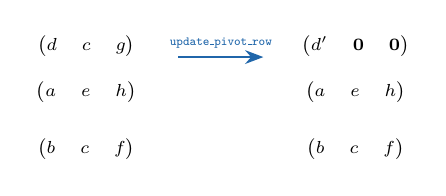
\begin{tikzpicture}[font=\scriptsize, every node/.style={transform shape}, scale=0.9]
			\node at (-1.9, 1) {$\begin{pmatrix} d & c & g \end{pmatrix}$};
			\node at (-1.9,  0.35) {$\begin{pmatrix} a & e & h \end{pmatrix}$};
			\node at (-1.9, -0.45) {$\begin{pmatrix} b & c & f \end{pmatrix}$};
			\node at ( 1.9, 1) {$\begin{pmatrix} d' & \mathbf{0} & \mathbf{0} \end{pmatrix}$};
			\node at ( 1.9,  0.35) {$\begin{pmatrix} a & e & h \end{pmatrix}$};
			\node at ( 1.9, -0.45) {$\begin{pmatrix} b & c & f \end{pmatrix}$};
			\draw[-{Stealth}, pivotblue, thick] (-0.6,0.85) -- (0.6,0.85)
		      node[midway, above] {\tiny \texttt{update\_pivot\_row}};
		\end{tikzpicture}
		
		\pause
		% -------- Update Kernel (RIGHT) ---------------------------------
		\column{0.48\textwidth}
		\begin{block}{2. Update Kernel – Apply the Transformation}
			\begin{itemize}\setlength{\itemsep}{3pt}
			  \item Receives parameters from the pivot kernel.
			  \item Applies the transformation to each trailing row.
			  \item Enables parallel execution across multiple rows.
			\end{itemize}
		\end{block}
		
		% mini-figure (two rows BEFORE → AFTER)
		\centering
		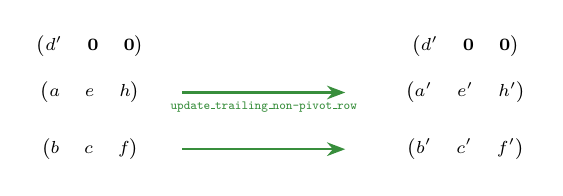
\begin{tikzpicture}[font=\scriptsize, every node/.style={transform shape}, scale=0.9]
			% before rows
			\node at (-2.1, 1) {$\begin{pmatrix} d' & \mathbf{0} & \mathbf{0} \end{pmatrix}$};
			\node at (-2.1,  0.35) {$\begin{pmatrix} a & e & h \end{pmatrix}$};
			\node at (-2.1, -0.45) {$\begin{pmatrix} b & c & f \end{pmatrix}$};
			% after rows
			\node at (3.2, 1) {$\begin{pmatrix} d' & \mathbf{0} & \mathbf{0} \end{pmatrix}$};
			\node at ( 3.2,  0.35) {$\begin{pmatrix} a' & e' & h' \end{pmatrix}$};
			\node at ( 3.2, -0.45) {$\begin{pmatrix} b' & c' & f' \end{pmatrix}$};
			% arrows
			\draw[-{Stealth}, updategreen, thick] (-0.8,  0.35) -- (1.5,  0.35)
			node[midway, below] {\tiny \texttt{update\_trailing\_non-pivot\_row}};
			\draw[-{Stealth}, updategreen, thick] (-0.8, -0.45) -- (1.5, -0.45);
		\end{tikzpicture}
	\end{columns}

	\pause
	\vspace{2mm}
	{\scriptsize \emph{The pivot kernel computes transformation parameters, which the update kernel applies to construct the upper-triangular matrix required by SLSQP.}}

\end{frame}        % The slide visualizing the kernels

% --- Placeholders for the rest of the presentation ---
% % Slide: Naive Barrier-Based Parallelism
% \begin{frame}{A Naive Approach: Parallelism with Barriers}
%   \begin{columns}[c,onlytextwidth] % Vertically center the columns

%     % ----- LEFT: The algorithm modified with a parallel loop and barriers -----
%     \column{0.55\textwidth}
%     \begin{block}{Barrier-Based Parallel Algorithm}
%       \footnotesize
%       \begin{algorithmic}[1]
%         \State \textbf{Input:} $A$, a $m \times n$ non-singular real matrix.
%         \For{$i = 1$ \textbf{to} $m$} \Comment{Outer loop remains sequential}
%           \State $(up, b) \gets \textcolor{pivotblue}{\Call{\texttt{update\_pivot\_row}}{A, i}}$
%           \State \textcolor{depred}{\textbf{--- BARRIER 1 ---}} \Comment{Wait for pivot to complete}
          
%           \ParallelFor{$j = i+1$ to $n$} \Comment{Parallelize row updates}
%             \State \textcolor{updategreen}{\Call{\texttt{update\_trailing\_non\_pivot\_row}}{A, i, j, up}}
%           \EndParallelFor
          
%           \State \textcolor{depred}{\textbf{--- BARRIER 2 ---}} \Comment{Wait for all updates to finish}
%         \EndFor
%         \State \textbf{Output:} Matrix $A$ in upper-triangular form.
%       \end{algorithmic}
%     \end{block}
% \end{columns}
%     % % ----- RIGHT: Explanation of the logic and its critical flaw -----
%     % \column{0.45\textwidth}
%     % \begin{block}{The Logic}
%     %   The most obvious way to parallelize the algorithm is to execute the inner loop across multiple threads. To maintain correctness:
%     %   \begin{itemize}
%     %     \item \textbf{Barrier 1} is needed to ensure the pivot data is ready before any thread can start an update.
%     %     \item \textbf{Barrier 2} is needed to ensure all row updates for iteration `i` are complete before we begin iteration `i+1`.
%     %   \end{itemize}
%     % \end{block}
    
%     % \begin{alertblock}{The Critical Flaw: Lost Performance}
%     %   This approach is inefficient. Threads that finish their work quickly are forced to \textbf{idle} at the barrier, waiting for the single \textbf{slowest thread} to catch up. This "tail waiting" is pure wasted time.
%     % \end{alertblock}
% \end{frame}


\begin{frame}{A Naive Approach: Parallelism with Barriers}
	
	\pause 
	\begin{columns}[c] % Vertically center the columns' content
	
	 % ----- LEFT: The algorithm -----
	 \begin{column}{0.55\textwidth}
	   \begin{block}{Barrier-Based Parallel Algorithm}
	     \footnotesize
	     \begin{algorithmic}[1]
	       \State \textbf{Input:} $A$, a $m \times n$ non-singular real matrix.
	       \For{$i = 1$ \textbf{to} $m$}
	         \State $(up, b) \gets \textcolor{pivotblue}{\Call{\texttt{update\_pivot\_row}}{A, i}}$
	         \State \textcolor{depred}{\textbf{--- BARRIER 1 ---}}
	         
	         \For{$j = i+1$ to $n$} \Comment{Parallel execution}
	           \State \textcolor{updategreen}{\Call{\texttt{update\_trailing\_non\_pivot\_row}}{A, i, j, up}}
	         \EndFor
	         
	         \State \textcolor{depred}{\textbf{--- BARRIER 2 ---}}
	       \EndFor
	       \State \textbf{Output:} Matrix $A$ in upper-triangular form.
	     \end{algorithmic}
	   \end{block}
	 \end{column}
	\end{columns}
\end{frame}
% Slide 4 — QR as a Task DAG (Updated with simplified alertblock bullets)
\begin{frame}{Problem Formulation: QR as a Task DAG}
	
	\pause 
	
	% Use [T] to top-align the columns for better control over vertical space
	\begin{columns}[c,onlytextwidth] 
		% ---------- LEFT: Content drastically condensed into a single block ----------
		\column{0.60\textwidth}
		\begin{block}{Task \& Dependency Model}
		  The QR algorithm is modeled as a DAG of tasks, $T_{i,j}$:
		  \begin{itemize}\setlength{\itemsep}{3pt} % Tighter item spacing
		    \item \textbf{Pivot Task ($T_{i,i}$):} Runs \texttt{update\_pivot\_row}.
		    \item \textbf{Update Task ($T_{i,j}, j>i$):} Runs \texttt{update\_trailing\_non\_pivot\_row}. % FIXED: Changed &gt; to > for LaTeX compatibility
		    \item \textbf{Dependencies:} A task $T_{i,j}$ can only run after its parents, \textbf{$T_{i,i}$} (pivot) and \textbf{$T_{i-1,j}$} (previous row), are complete.
		  \end{itemize}
		\end{block}
	
		\pause 
		\begin{alertblock}{Scheduling Goal}
		  \begin{itemize}\setlength{\itemsep}{3pt} % Keep bullets tight to fit page
		    \item Execute the task DAG in parallel.
		    \item Respect all task dependencies.
		    %\item Avoid the overhead caused by global synchronization barriers.
		  \end{itemize}
		\end{alertblock}
	
		% ---- Right: TaskGraph figure with adjusted scale and caption ----		
		\column{0.40\textwidth}
		\centering
		\definecolor{lightblue}{RGB}{173, 216, 230}
		
		% --- Further reduced scale to guarantee fit ---
		\pause 
		\begin{tikzpicture}[node distance=1cm and 0.5cm, scale=0.5, transform shape]
			% Nodes - Row 1
			\node[draw, circle, fill=lightblue] (T11) at (0,0) {$T_{1,1}$};
			\node[draw, circle, fill=lightblue] (T12) at (1.4,-1.2) {$T_{1,2}$};
			\node[draw, circle] (T13) at (2.6,-1.2) {$T_{1,3}$};
			\node[draw, circle] (T14) at (3.8,-1.2) {$T_{1,4}$};
			\node[draw, circle] (T15) at (4.9,-1.2) {$T_{1,5}$};
			
			% Nodes - Row 2
			\node[draw, circle, fill=lightblue] (T22) at (1.4,-2.5) {$T_{2,2}$};
			\node[draw, circle, fill=lightblue] (T23) at (2.6,-3.5) {$T_{2,3}$};
			\node[draw, circle] (T24) at (3.8,-3.5) {$T_{2,4}$};
			\node[draw, circle] (T25) at (4.9,-3.5) {$T_{2,5}$};
			
			% Nodes - Row 3
			\node[draw, circle, fill=lightblue] (T33) at (2.6,-4.8) {$T_{3,3}$};
			\node[draw, circle, fill=lightblue] (T34) at (3.8,-5.8) {$T_{3,4}$};
			\node[draw, circle] (T35) at (4.9,-5.8) {$T_{3,5}$};
			
			% Nodes - Row 4
			\node[draw, circle, fill=lightblue] (T44) at (3.8,-7.1) {$T_{4,4}$};
			\node[draw, circle, fill=lightblue] (T45) at (4.9,-8.1) {$T_{4,5}$};
			
			% Nodes - Row 5
			\node[draw, circle, fill=lightblue] (T55) at (4.9,-9.7) {$T_{5,5}$};
			
			% Edges (condensed to save space in the .tex file)
			\draw[->] (T11) -- (T12); \draw[->] (T12) -- (T22); \draw[->] (T13) -- (T23);
			\draw[->] (T14) -- (T24); \draw[->] (T15) -- (T25); \draw[->, bend left] (T11) to (T13);
			\draw[->, bend left] (T11) to (T14); \draw[->, bend left] (T11) to (T15);
			\draw[->] (T22) -- (T23); \draw[->] (T24) -- (T34); \draw[->] (T25) -- (T35);
			\draw[->, bend left] (T22) to (T24); \draw[->, bend left] (T22) to (T25);
			\draw[->] (T23) -- (T33); \draw[->, bend left] (T33) to (T34); \draw[->, bend left] (T33) to (T35);
			\draw[->] (T34) -- (T44); \draw[->] (T35) -- (T45); \draw[->, bend left] (T44) to (T45);
			\draw[->] (T45) -- (T55);
		\end{tikzpicture}
		
		% --- Added the requested figure caption ---
		\vspace{1mm}
		{\scriptsize \emph{TaskGraph for Triangular System}}
	
	\end{columns}
\end{frame}

% ------------------------------------------------------------------
% Slide: Barrier-Based Task Scheduling (concise version)
% ------------------------------------------------------------------
\begin{frame}{List Scheduling with Barriers}
	\pause 
	\begin{columns}[c,onlytextwidth]
	
	% ----- LEFT: Barrier logic ------------------------------------
	\column{0.50\textwidth}
	\begin{block}{The Barrier-Based Approach}
	  \begin{itemize}\setlength{\itemsep}{3pt}
	    \item Model QR as a graph of tasks ($T_{i,j}$).
	    \item \textbf{Barrier 1}: All threads wait after pivot task ($T_{i,i}$) is completed.
	    \item \textbf{Barrier 2}: All threads wait after all update tasks ($T_{i,j}$) finish before the next iteration.
	  \end{itemize}
	\end{block}
	
	% ----- RIGHT: Critical flaw text + figure ---------------------
	\pause	
	\column{0.45\textwidth}
	\begin{alertblock}{Why Barriers Hurt Performance}
		\begin{itemize}\setlength{\itemsep}{3pt}
		 \item Barriers force strictly synchronous execution.
		 \item Faster threads idle while the slowest thread finishes.
		 \item The idle time reduces overall throughput.
		\end{itemize}
	\end{alertblock}
	\end{columns}
	
	\pause
	\begin{columns}
	\column{0.70\textwidth}
	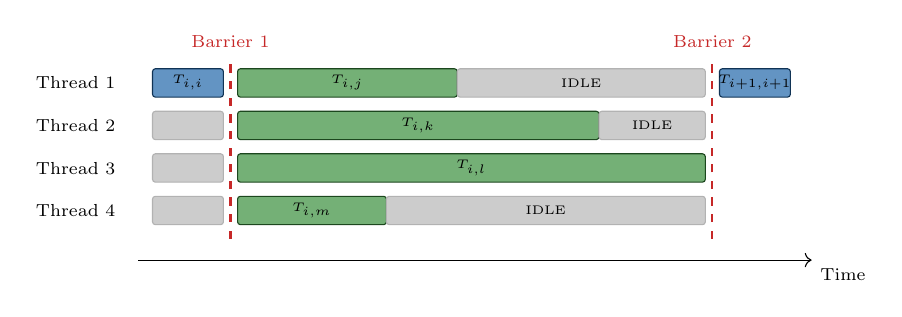
\begin{tikzpicture}[font=\tiny, every node/.style={transform shape}, scale=0.90]
		% Styles for different states
		\tikzset{pivot/.style={fill=pivotblue!70, draw=pivotblue!50!black, rounded corners=1pt}}
		\tikzset{work/.style={fill=updategreen!70, draw=updategreen!50!black, rounded corners=1pt}}
		\tikzset{wait/.style={fill=gray!40, draw=gray!60, rounded corners=1pt}}
		\tikzset{bar/.style={draw=depred, thick, dashed}}
		
		% Time Axis
		\draw[->] (0,0) -- (9.5,0) node[anchor=north west, font=\scriptsize] {Time};
		
		% Thread Labels
		\node[anchor=east, font=\scriptsize] at (-0.2, 2.5) {Thread 1};
		\node[anchor=east, font=\scriptsize] at (-0.2, 1.9) {Thread 2};
		\node[anchor=east, font=\scriptsize] at (-0.2, 1.3) {Thread 3};
		\node[anchor=east, font=\scriptsize] at (-0.2, 0.7) {Thread 4};
		
		% --- Iteration i with new, narrower coordinates ---
		\draw[pivot] (0.2, 2.3) rectangle node{$T_{i,i}$} (1.2, 2.7);
		\draw[wait]  (0.2, 1.7) rectangle (1.2, 2.1);
		\draw[wait]  (0.2, 1.1) rectangle (1.2, 1.5);
		\draw[wait]  (0.2, 0.5) rectangle (1.2, 0.9);
		\node[above=2pt, depred, font=\scriptsize] at (1.3, 2.8) {Barrier 1};
		\draw[bar] (1.3, 0.3) -- (1.3, 2.8);
		
		\draw[work] (1.4, 2.3) rectangle node{$T_{i,j}$} (4.5, 2.7);
		\draw[work] (1.4, 1.7) rectangle node{$T_{i,k}$} (6.5, 2.1);
		\draw[work] (1.4, 1.1) rectangle node{$T_{i,l}$} (8.0, 1.5); % SLOWEST
		\draw[work] (1.4, 0.5) rectangle node{$T_{i,m}$} (3.5, 0.9);
		
		\draw[wait] (4.5, 2.3) rectangle node{\textcolor{black}{IDLE}} (8.0, 2.7);
		\draw[wait] (6.5, 1.7) rectangle node{\textcolor{black}{IDLE}} (8.0, 2.1);
		\draw[wait] (3.5, 0.5) rectangle node{\textcolor{black}{IDLE}} (8.0, 0.9);
		
		\node[above=2pt, depred, font=\scriptsize] at (8.1, 2.8) {Barrier 2};
		\draw[bar] (8.1, 0.3) -- (8.1, 2.8);
		
		\draw[pivot] (8.2, 2.3) rectangle node{$T_{i+1,i+1}$} (9.2, 2.7);
	\end{tikzpicture}
	
	\column{0.25\textwidth}
	{\scriptsize \emph{Fig : Global barriers introduce idle time and squander parallel resources.}}
	\end{columns}

\end{frame}

% Slide: The Two-Queue Logic (Corrected and Redesigned)
\tikzstyle{startstop} = [rectangle, rounded corners, minimum width=3cm, minimum height=1cm, text centered, draw=black]
\tikzstyle{process} = [rectangle, minimum width=3cm, minimum height=1cm, text centered, draw=black]
\tikzstyle{decision} = [diamond, minimum width=3cm, minimum height=0.8cm, text centered, draw=black]
\tikzstyle{arrow} = [thick,->,>=stealth]

\begin{frame}{Our Solution: The Two-Queue Logic}
  
	\begin{columns}[c,onlytextwidth] % Vertically centered
			
		% ----- LEFT: The text explaining the diagram -----
		\pause 
		\column{0.45\textwidth}
		\begin{alertblock}{The Two-Queue Flow}
			The scheduler's logic is a simple loop:
			\begin{itemize}
		 \item A thread dequeues a task from the \textbf{Main Queue} and executes it.
		 \item Then it checks if the dependencies are satisfied for its child tasks.
		 \item \textbf{If YES:} The child task is enqueued in the main queue.
		 \item \textbf{If NO:} The child task is enqueued to the \textbf{Wait Queue} to be re-checked again by any thread.
			\end{itemize}
		\end{alertblock}
		
		% ----- RIGHT: The new, clean, and compact diagram -----
		\pause 
		\column{0.55\textwidth}
		% First Diagram
		\centering
		\begin{tikzpicture}[node distance=1.8cm, scale=0.7, transform shape, xshift=0cm]
	  
		 % Nodes
		 \node (root) [startstop, fill=red!30] {Root Node};
		 \node (mq) [process, below of=root, fill=blue!30] {Main Queue};
		 \node (executor) [process, below of=mq, fill=green!30] {Executor};
		 \node (dep) [decision, right of=executor, xshift=3cm, fill=yellow!30] {Dep Satisfied? };
		 \node (wq) [process, below of=dep, yshift=-2cm, fill=purple!30] {Wait Queue};
		 \node (terminate) [startstop, below of=executor, yshift=-2cm, fill=orange!30] {Terminate};
		 
		 % Arrows
		 \draw [arrow] (root) -- node[right] {Enqueue} (mq);
		 \draw [arrow] (mq) -- node[right] {Dequeue} (executor);
		 \draw [arrow] (executor.east) -- node[above] {If children} (dep.west);
		 \draw [arrow] (executor.south) -- node[right] {If no children} (terminate.north);
		 
		 % Rectangular arrow for "No" path
		 \draw [arrow] (dep.east) -- node[above] {No} ++(0.5,0) --node[midway,left] {Enqueue} ++(0,-3.8) -- (wq.east);
		 
		 % Arrow back from WQ
		 \draw [arrow] (wq.west) -- ++(-0.5,0) -- ++(-0.3, 0) -- node[midway,right] {Dequeue} ++(0.0, 2) -- ++(2.3,0) -- (dep.south);
		 
		 % "Yes" path looping back to MQ
		 \draw [arrow] (dep.north) |- node[right] {Yes} (mq.east) node[right, above]{\quad\quad\quad\quad\quad\quad\quad\quad Enqueue};  
		\end{tikzpicture}
	\end{columns}
\end{frame}
% Simulation Slide 1: The Initial State
\begin{frame}{Simulation: The Two-Queue Scheduler in Action}
  \begin{columns}[c,onlytextwidth] % Vertically centered

    % ----- LEFT: The text explaining the current state -----
    \column{0.4\textwidth}
    \begin{block}{Let's Begin the Simulation}
      The system starts with all threads idle in the pool and both queues empty.
    \end{block}

    \begin{alertblock}<2->{State A: Initial Task}
      The first pivot task, \textbf{$T_{1,1}$}, is the only task with no dependencies.
      \vspace{2mm}
      It is placed at the \textbf{front} of the Main Queue, ready to be dequeued.
    \end{alertblock}

    % ----- RIGHT: The diagram showing the initial state -----
    \column{0.6\textwidth}
    \centering
    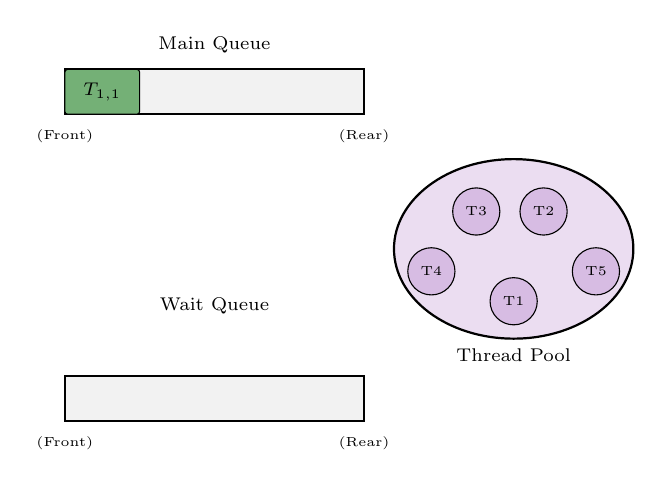
\begin{tikzpicture}[font=\scriptsize, every node/.style={transform shape}, scale=0.95]
      % Styles
      \tikzset{pool/.style={draw, thick, ellipse, fill=accent!15, minimum width=3.2cm, minimum height=2.4cm, align=center}}
      \tikzset{thread_icon/.style={draw, circle, fill=accent!30, minimum size=0.5cm}}
      \tikzset{task_ready/.style={draw, rectangle, rounded corners=1pt, fill=updategreen!70, minimum width=1cm, minimum height=0.6cm}}
      \tikzset{queue_box/.style={draw, thick, fill=gray!10}}
      
      % --- The Worker Thread Pool ---
      \node[pool] (pool) at (2.5, 0) {};
      \node[thread_icon] at ($(pool.center)+(0, -0.7)$) {\tiny T1};
      \node[thread_icon] at ($(pool.center)+(0.4,0.5)$) {\tiny T2};
      \node[thread_icon] at ($(pool.center)+(-0.5, 0.5)$) {\tiny T3};
      \node[thread_icon] at ($(pool.center)+(-1.1, -0.3)$) {\tiny T4};
      \node[thread_icon] at ($(pool.center)+(1.1, -0.3)$) {\tiny T5};
      \node[anchor=north] at (pool.south) {Thread Pool};

      % --- The Queues ---
      \node[anchor=south] at (-1.5, 2.5) {Main Queue};
      \draw[queue_box] (-3.5, 1.8) rectangle (0.5, 2.4);
      \node[font=\tiny] at (-3.5, 1.5) {(Front)};
      \node[font=\tiny] at (0.5, 1.5) {(Rear)};
      \node[anchor=south] at (-1.5, -1.0) {Wait Queue};
      \draw[queue_box] (-3.5, -1.7) rectangle (0.5, -2.3);
      \node[font=\tiny] at (-3.5, -2.6) {(Front)};
      \node[font=\tiny] at (0.5, -2.6) {(Rear)};

      % --- Animation: The initial task appears on the second click ---
      \node<2->[task_ready] at (-3, 2.1) {$T_{1,1}$};
      
    \end{tikzpicture}
  \end{columns}
\end{frame}
\begin{frame}{Simulation: The Two-Queue Scheduler in Action}
  \begin{columns}[c,onlytextwidth] % Vertically centered

    % ----- LEFT: The text explaining State B -----
    \column{0.4\textwidth}
    \begin{alertblock}{State B: Execution \& Spawning}
      An idle thread, \textbf{T1}, dequeues the pivot task \textbf{$T_{1,1}$} from the \textbf{front} of the Main Queue.
      \vspace{2mm}
      
      After executing it, T1 enqueues the newly spawned, ready-to-run child tasks (\textbf{$T_{1,2}, T_{1,3}, \dots$}) to the \textbf{rear} of the Main Queue.
    \end{alertblock}

    % ----- RIGHT: The diagram showing the action of State B -----
    \column{0.6\textwidth}
    \centering
    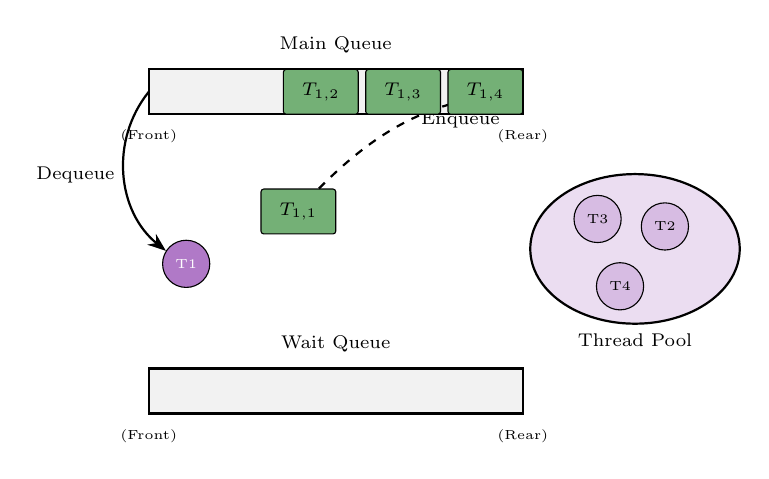
\begin{tikzpicture}[font=\scriptsize, every node/.style={transform shape}, scale=0.95]
      % Styles
      \tikzset{pool/.style={draw, thick, ellipse, fill=accent!15, minimum width=2.8cm, minimum height=2cm, align=center}}
      \tikzset{thread_icon/.style={draw, circle, fill=accent!30, minimum size=0.5cm}}
      \tikzset{active_thread/.style={thread_icon, fill=accent!60, text=white, minimum size=0.6cm}}
      \tikzset{task_ready/.style={draw, rectangle, rounded corners=1pt, fill=updategreen!70, minimum width=1cm, minimum height=0.6cm}}
      \tikzset{queue_box/.style={draw, thick, fill=gray!10}}
      
      % --- Repositioned Elements for Clarity ---
      % Main Queue at the top
      \node[anchor=south] at (-0.5, 2.5) {Main Queue};
      \draw[queue_box] (-3, 1.8) rectangle (2, 2.4);
      \node[font=\tiny] at (-3, 1.5) {(Front)};
      \node[font=\tiny] at (2, 1.5) {(Rear)};

      % Wait Queue at the bottom
      \node[anchor=south] at (-0.5, -1.5) {Wait Queue};
      \draw[queue_box] (-3, -2.2) rectangle (2, -1.6);
      \node[font=\tiny] at (-3, -2.5) {(Front)};
      \node[font=\tiny] at (2, -2.5) {(Rear)};

      % Thread Pool on the right (T1 is missing)
      \node[pool] (pool) at (3.5, 0) {};
      \node[thread_icon] at ($(pool.center)+(0.4,0.3)$) {\tiny T2};
      \node[thread_icon] at ($(pool.center)+(-0.5, 0.4)$) {\tiny T3};
      \node[thread_icon] at ($(pool.center)+(-0.2, -0.5)$) {\tiny T4};
      \node[anchor=north] at (pool.south) {Thread Pool};

      % --- Active T1 and its task are in the center-left "workspace" ---
      \node[active_thread] (active_t1) at (-2.5, -0.2) {\tiny T1};
      \node[task_ready] (task_t11) at (-1, 0.5) {$T_{1,1}$};

      % --- The Actions (Clear, Curved Arrows) ---
      % Dequeue Arrow: from Front of Queue to the active T1
      \draw[-{Stealth}, thick] (-3, 2.1) to[bend right=45] node[midway, left] {Dequeue} (active_t1);
      
      % Enqueue Arrow: from the processed task to the Rear of Queue
      \draw[-{Stealth}, thick, dashed] (task_t11) to[bend left=20] node[midway, right] {Enqueue} (2, 2.1);
      
      % --- The Result: New tasks are now in the Main Queue ---
      \node[task_ready] at (1.5, 2.1) {$T_{1,4}$};
      \node[task_ready] at (0.4, 2.1) {$T_{1,3}$};
      \node[task_ready] at (-0.7, 2.1) {$T_{1,2}$};
      
    \end{tikzpicture}
  \end{columns}
\end{frame}
% Simulation Slide 3, Step 1: The Initial State (Final Revised Version)
\begin{frame}{Simulation: Navigating the Dependency Graph}
  \begin{columns}[c,onlytextwidth]

    % ----- LEFT: Text for the initial state -----
    \column{0.38\textwidth}
    \only<1>{
      \begin{alertblock}{Mid-Execution Step}
      After executing $T_{2, 2}$ its children's dependencies are checked and enqueued to the main queue if its dependency is satisfied or else its enqueued into the wait queue.
        
      \end{alertblock}
    }
    \only<2>{
      \begin{alertblock}{Step 5: Dependency Aware Enqueue Process}
        Thread \textbf{T3} is processing its task from the previous level.
        So the children task $T_{2, 4}$ gets pushed to the wait queue as its parent task is incomplete.
      \end{alertblock}
    }
    \only<3>{
      \begin{alertblock}{Step 6: Continued Execution with Readily Available Tasks}
        The remaining threads can pick up other immediately executable tasks from the main queue.
      \end{alertblock}
    }
        \only<4>{
      \begin{alertblock}{Step 7: Next Pivot Push}
        \textbf{T1} finishes $T_{2, 3}$ and enqueues its child, the new pivot \textbf{$T_{3,3}$}. Also, $T_{1, 4}$ is complete in the mean time so its child $T_{2, 4}$ can be safely pushed to the main queue.
    \end{alertblock}
    }
        \only<5>{
      \begin{alertblock}{Step 8: Promotion Admist Work}
        Since, the parent of $T_{2, 4}$ was complete, $T_{2, 4}$ got promoted from the wait queue to the main queue as an immediately executable task.
      \end{alertblock}
    }

        \only<6>{
      \begin{alertblock}{Step 9: Further Execution with Immediately Executable Tasks}
        The threads can pick up more executable tasks from the main queue and continue executing the nodes of the DAG in a non-blocking manner.
      \end{alertblock}
    }


    % ----- RIGHT: The static diagram with your new layout and dashed arrows -----
    \column{0.61\textwidth}
    \centering
    \begin{tikzpicture}[font=\scriptsize, every node/.style={transform shape}, scale=0.95]
      % Styles
      \tikzset{pool/.style={draw, thick, ellipse, fill=accent!15, minimum width=2.8cm, minimum height=2cm}}
      \tikzset{thread_icon/.style={draw, circle, fill=accent!30, minimum size=0.5cm}}
      \tikzset{active_thread/.style={thread_icon, fill=accent!60, text=white, minimum size=0.6cm}}
      \tikzset{task_ready/.style={draw, rectangle, rounded corners=1pt, fill=updategreen!70, minimum width=1cm, minimum height=0.6cm}}
      \tikzset{task_wait/.style={draw, rectangle, rounded corners=1pt, fill=gray!50, minimum width=1cm, minimum height=0.6cm}}
      \tikzset{queue_box/.style={draw, thick, fill=gray!10, minimum width=5cm, minimum height=0.8cm}}
      
      % --- Layout Elements ---
      \node[pool] (pool) at (3.5, 0) {}; \node[anchor=north] at (pool.south) {Thread Pool};
      \node[queue_box] (mainq) at (-0.5, 2.1) {}; \node[anchor=south] at (mainq.north) {Main Queue};
      \node[font=\tiny] at ([yshift=-0.3cm]mainq.south west) {(Front)}; \node[font=\tiny] at ([yshift=-0.3cm]mainq.south east) {(Rear)};
      \node[queue_box] (waitq) at (-0.5, -2.1) {}; \node[anchor=north] at ([yshift=0.4cm]waitq.north) {Wait Queue};
      \node[font=\tiny] at ([yshift=-0.3cm]waitq.south west) {Front)}; \node[font=\tiny] at ([yshift=-0.3cm]waitq.south east) {(Rear)};
      
      % --- Initial State Elements ---
       \only<1>{
      % Active Threads (T3 and T4)
      \node[active_thread] (t3) at (0, 0.7) {\tiny T3}; \node[task_ready, right=1mm of t3] {$T_{1,4}$};
      \node[active_thread] (t4) at (0, -0.7) {\tiny T4}; \node[task_ready, right=1mm of t4] {$T_{1,5}$};
      
      \node[thread_icon] (t2_idle) at ($(pool.center)+(0,0.5)$) {\tiny T2};
      
      % Tasks in Main Queue
      \node[task_ready] (t22_q) at ([xshift=-1.8cm]mainq.center) {$T_{2,2}$};
          \node[active_thread] (active_t1) at (-2.5, -0.7) {\tiny T1};
        \draw[-{Stealth}, thick] (mainq.west) to[bend right=60] node[midway, left] {Dequeue} (active_t1);

      }


 % --- STATE 2 (After First Click - Corrected) ---


      % --- STATE 3 (After Second Click - Corrected) ---
      \only<2>{
        % T3 is still active, executing the parent task
        \node[active_thread] (t3) at (0, 0.7) {\tiny T3}; \node[task_ready, right=1mm of t3] {$T_{1,4}$};
        \node[active_thread] (active_t2) at (-2.5, -0.7) {\tiny T1};
        % The fail arrow appears, and T2,4 moves to the Wait Queue
    
        \node[task_wait] (t24_q)at ([xshift=1.8cm]waitq.center) {$T_{2,4}$};
        \draw[-{Stealth}, thick, depred, dashed] (active_t2) to[out=180, in=220] 
        node[midway, below left] {Fail} (t24_q.south);
        \node[task_ready] (t23_q) at ([xshift=0.6cm]mainq.west) {$T_{2,3}$};
        \node[task_ready] (t25_q) at ([xshift=1.6cm]mainq.west) {$T_{2,5}$};
          \node[thread_icon] (t4_idle) at ($(pool.center)+(0,-0.5)$) {\tiny T4};
        \node[thread_icon] (t2_idle) at ($(pool.center)+(0,0.5)$) {\tiny T2};   
         \draw[-{Stealth}, thick, dashed] (active_t1) to[bend right=60] 
        node[midway, below right] {Pass} (t25_q.east);

      }
      % --- STATE 4 (After Third Click) ---
      \only<3>{
        \node[active_thread] (t3) at (0, 0.7) {\tiny T3}; \node[task_ready, right=1mm of t3] {$T_{1,4}$};
        \node[thread_icon] at ($(pool.center)+(0.8,0.2)$) {\tiny T4};
       
        \node[active_thread] (active_t1) at (-2.5, -0.7) {\tiny T1};
        \draw[-{Stealth}, thick] (mainq.west) to[bend right=60] node[midway, left] {Dequeue} (active_t1);

        \node[active_thread] (active_t2) at (-1.5, -0.7) {\tiny T2};
        
        \node[task_ready] (t23_q) at ([xshift=0.6cm]mainq.west) {$T_{2,3}$};

        \node[task_ready] (t25_q) at ([xshift=1.6cm]mainq.west) {$T_{2,5}$};
    
        % T2,4 is still in the Wait Queue
        \node[task_wait] at ([xshift=1.8cm]waitq.center) {$T_{2,4}$};
        
      \draw[-{Stealth}, thick] (t25_q.east) to[bend left=60]  (active_t2);
      }
      % --- STATE 5 (After Fourth Click) ---
      \only<4>{
       

        \node[thread_icon] at ($(pool.center)+(0.8,0.2)$) {\tiny T3};
        \node[thread_icon] at ($(pool.center)+(-0.5,-0.5)$) {\tiny T4};
        \node[active_thread] (active_t2) at (-2.5, -0.7) {\tiny T2};
        \node[task_ready, right=1mm of active_t2] {$T_{2,5}$};

        \node[task_ready] at ([xshift=-0.8cm]mainq.east) {$T_{3,3}$};

        \node[active_thread] (t3) at (0, 0.7) {\tiny T1}; 
        \draw[-{Stealth}, thick] (0.3, 0.7) to[bend right=30] node[midway, right] {enqueue}([xshift=1.4cm]mainq.south);
        
        \node[task_ready] at ([xshift=0.8cm]waitq.west) {$T_{2,4}$};
      }

      \only<5>{
        % T1 and T3 are idle

        \node[thread_icon] at ($(pool.center)+(0.8,0.2)$) {\tiny T4};
        \node[thread_icon] at ($(pool.center)+(0.1,0.2)$) {\tiny T2};

        \node[active_thread] (active_t2) at (-2.5, -0.7) {\tiny T1};

        \draw[-{Stealth}, thick, updategreen, dashed] (waitq.west) to[bend left =45] (active_t2);
        \draw[-{Stealth}, thick, updategreen, dashed] (active_t2) to[bend right=30] node[midway, left] {Promote} ([xshift = 1.6cm]mainq.south);
        \node[task_ready] at ([xshift=1.8cm]mainq.center) {$T_{2,4}$};

      \node[active_thread] (t4) at (0, -0.7) {\tiny T3}; \node[task_ready, right=1mm of t4] {$T_{3,3}$};
      }

      % --- STATE 7 (After Sixth Click) ---
    \only<6->{
        % Idle threads remaining in the pool
        \node[thread_icon] at ($(pool.center)+(-0.8,0.2)$) {\tiny T3};
        
        % T2 and T4 are now active, taking the NEW work
        \node[active_thread] (active_t2) at (-2.5, -0.7) {\tiny T1};
        \node[active_thread] (active_t1) at (0, -0.7) {\tiny T4};
        \node[active_thread] (active_t3) at (-3.5, 0.7) {\tiny T2};
        
        % Arrows showing T2 and T4 dequeuing the new tasks
        \draw[-{Stealth}, thick] ([xshift=0.4cm]mainq.center) to[bend right = 15] (active_t2);
        \draw[-{Stealth}, thick] ([xshift=1.8cm]mainq.center) to[bend right] (active_t1);
        \draw[-{Stealth}, thick] ([xshift=0.4cm]mainq.west) to[bend right = 45] (active_t3);
        % T3 has implicitly finished T3,3 and enqueued its children
        % The children are now in the main queue
        \node[task_ready] at ([xshift=0.4cm]mainq.center) {$T_{3,4}$};
        \node[task_ready] at ([xshift=1.8cm]mainq.center) {$T_{3,5}$};
        
        % T2,4 is also still in the queue, ready to be picked up
        \node[task_ready] at ([xshift=-1.8cm]mainq.center) {$T_{2,4}$};
        
        }
      
\end{tikzpicture}
\end{columns}
\end{frame}
% \input{Slide_Results.tex}
% \input{Slide_RelatedWork.tex}
% \input{Slide_Conclusion.tex}
% \input{Slide_ThankYou.tex}


\end{document}